\documentclass[10pt,a4paper]{article}
\usepackage[utf8]{inputenc}
\usepackage[T1]{fontenc}
\usepackage{lmodern}
\usepackage{microtype}
\usepackage{geometry}
\geometry{a4paper, margin=1in}
\usepackage{tikz}
\usetikzlibrary{positioning, arrows.meta, shapes.geometric, calc}
\usepackage{hyperref}
\usepackage{enumitem}
\usepackage{titlesec}
\usepackage{parskip}
\usepackage{xcolor}
\usepackage{graphicx}
\usepackage{listings}
\usepackage{amsmath}

\lstset{
    % basicstyle=\ttfamily\scriptsize,
    breaklines=true,
    frame=single,
    backgroundcolor=\color{gray!5},
    keywordstyle=\color{blue},
    stringstyle=\color{red},
    commentstyle=\color{green!50!black}
}

\title{\textbf{G-ABM: Generative Agent-Based Macro-Simulation Engine for Financial Panic Dynamics}}
\author{Benjamin Förster}
\date{\today}

\begin{document}

\maketitle

\vspace{0.5cm}

\noindent \textbf{Track:} MLOps / LLMOps Systems Engineering \\
\textbf{Difficulty Level:} 08/10 \\
\textbf{Target Execution Budget:} \$0.00 (100\% Local Inference via Heterogeneous CPU/GPU Compute) \\
\textbf{Primary Focus:} Production Pipeline Engineering, Distributed Agent Orchestration, Systemic Drift Monitoring, and Local LLM Serving Optimisation.

\vspace{0.5cm}
\begin{abstract}
\noindent Traditional Agent-Based Models rely on rigid heuristics that fail to capture the bounded rationality and emotional contagion of real human populations during crisis events. While Large Language Models offer unprecedented cognitive realism, their latency prevents their use in massive-scale environments. To solve this, this project introduces a hybrid generative macro-simulation engine. The system establishes a stable financial equilibrium using algorithmic, Inventory-Aware Market Makers to provide continuous liquidity. Into this baseline, a swarm of generative LLM agents is injected to act as disruptive, panic-susceptible retail and institutional traders. By broadcasting macroeconomic shocks to the LLM swarm and measuring their subsequent irrational trading behaviour against the algorithmic equilibrium, the system simulates liquidity crises and flash crashes. The architecture relies on rigorous MLOps engineering to sustain massive asynchronous concurrency locally on consumer hardware.
\end{abstract}
\vspace{0.5cm}

\section{Introduction}

The systemic collapse of a financial market during a flash crash is rarely driven by the rational equilibrium equations found in traditional economic models. Instead, it is an emergent phenomenon driven by messy, profoundly human factors: a rumour propagating through a retail trading forum, the sudden emotional panic of over-leveraged day traders, and the relentless, cascading liquidations triggered by institutional algorithms.

To simulate these highly volatile, tail-risk events realistically, we must move beyond hard-coded agent logic. This project builds a system to model irrational human panic at scale. A core challenge in multi-agent generative environments is model collapse, where irrational LLM actions instantly drain market liquidity and halt the simulation. To prevent this, the simulation relies on a robust market microstructure: continuous, algorithmic Inventory-Aware Market Makers provide a mathematical baseline of bid and ask liquidity, dynamically widening spreads to defend against toxic flow.

Into this stable equilibrium, small patches of the population are simulated using generative LLM agents. These models actively read breaking news from a central orchestrator, interpret the depth of a crashing limit order book, and generate nuanced, internal reasoning traces before taking action, such as panic selling. The primary benchmarking scenario involves measuring exactly how much irrational LLM herd behaviour is required to overwhelm the algorithmic market makers and trigger a systemic flash crash. This allows for the rigorous testing of MLOps pipelines under extreme asynchronous concurrency.

\section{Logical Target Architecture}

\begin{figure}[t]
\centering
\resizebox{0.5\textwidth}{!}{%
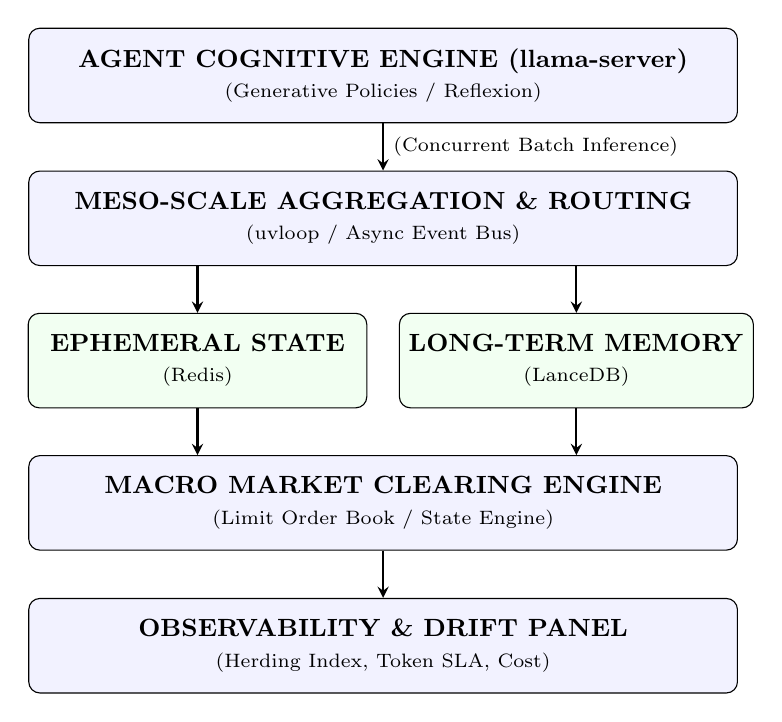
\begin{tikzpicture}[
    box/.style={draw, rectangle, rounded corners, minimum width=9cm, minimum height=1.2cm, align=center, fill=blue!5, font=\small},
    smallbox/.style={draw, rectangle, rounded corners, minimum width=4.3cm, minimum height=1.2cm, align=center, fill=green!5, font=\small},
    arrow/.style={->, >=stealth, thick}
]

% Nodes
\node[box] (agent) {\textbf{AGENT COGNITIVE ENGINE (llama-server)}\\ \scriptsize (Generative Policies / Reflexion)};
\node[box, below=0.6cm of agent] (meso) {\textbf{MESO-SCALE AGGREGATION \& ROUTING}\\ \scriptsize (uvloop / Async Event Bus)};

% Calculate center points for the two smaller boxes
\coordinate (center) at ($(meso.south) + (0,-1.2cm)$);
\node[smallbox, left=0.2cm of center] (redis) {\textbf{EPHEMERAL STATE}\\ \scriptsize (Redis)};
\node[smallbox, right=0.2cm of center] (lancedb) {\textbf{LONG-TERM MEMORY}\\ \scriptsize (LanceDB)};

\node[box, below=1.2cm of center] (macro) {\textbf{MACRO MARKET CLEARING ENGINE}\\ \scriptsize (Limit Order Book / State Engine)};
\node[box, below=0.6cm of macro] (observability) {\textbf{OBSERVABILITY \& DRIFT PANEL}\\ \scriptsize (Herding Index, Token SLA, Cost)};

% Edges
\draw[arrow] (agent) -- node[right, align=left] {\scriptsize (Concurrent Batch Inference)} (meso);
\draw[arrow] (meso.south -| redis.north) -- (redis.north);
\draw[arrow] (meso.south -| lancedb.north) -- (lancedb.north);
\draw[arrow] (redis.south) -- (redis.south |- macro.north);
\draw[arrow] (lancedb.south) -- (lancedb.south |- macro.north);
\draw[arrow] (macro) -- (observability);

\end{tikzpicture}%
}
\caption{Logical Target Architecture mapping the Generative Agents to the Event Bus and LOB.}
\label{fig:logical_arch}
\end{figure}

As illustrated in Figure \ref{fig:logical_arch}, the system operates as a continuous feedback loop across several decoupled layers. This architecture ensures that the slow, non-deterministic generation of the language models does not block the high-speed execution of the financial matching engine. 

\textbf{Agent Cognitive Engine (llama-server):} At the top of the stack, the generative LLM agents reside. These agents receive the latest market state as a single, shared prompt prefix. Utilising the llama-server inference engine, the agents evaluate their individual personas and risk tolerances to generate discrete trading decisions. A built-in reflexion loop acts as an internal cognitive critique, forcing agents to evaluate their proposed actions against their historical behaviour before emitting the final structured JSON payload.

\textbf{Meso-Scale Aggregation and Routing (uvloop):} Because up to 400 agents generating actions asynchronously per tick would overwhelm standard Python event loops, a Cython-based \texttt{uvloop} event bus acts as the central nervous system. It ingests the JSON payloads from the cognitive engine, validates the schemas, and batches the orders into discrete temporal windows (simulation ticks). Crucially, simulation time is decoupled from wall-clock time: the LOB clock advances from tick $t$ to $t+1$ only after the full asynchronous agent batch has been collected. This preserves causal integrity without imposing a physically impossible real-time latency SLA.

\textbf{State Management (Redis and LanceDB):} The event bus relies on a bifurcated memory architecture to manage state. Because tick snapshots are injected directly into the Radix prompt prefix at the start of each tick, mid-tick Redis read operations are eliminated. Redis acts exclusively as a write-sink and tick-boundary coordination ledger: at the $t+1$ tick boundary, the clearing engine writes the final executed prices, inventory snapshots, and market maker state to Redis, from which the event bus assembles the next tick's prompt prefix. Conversely, LanceDB acts as a persistent vector store on disk. It continuously archives the textual reasoning traces generated by the agents during their reflexion phase, allowing for long-term semantic retrieval and post-simulation behavioural analysis.

\textbf{Macro Market Clearing Engine:} At the core of the financial simulation lies a compiled, memory-contiguous Limit Order Book (LOB) matching engine. It receives the batched orders from the event bus and executes price-time priority matching. By strictly separating the heavy string manipulation of the LLMs from the pure numerical array operations of the clearing engine, the system maintains a mathematically sound equilibrium. 

\textbf{Observability and Drift Panel:} Finally, the clearing engine outputs the derived asset prices and agent execution logs to a telemetry stack. This observability layer tracks critical systems metrics, such as generation latency, alongside emergent financial metrics, including the herding index, which quantifies the exact moment the LLM swarm overwhelms the algorithmic market makers.

\section{Server Setup \& Hardware Provisioning}

As the deployment necessitates executing real-time multi-agent inference strictly within the 16GB GDDR7 VRAM boundary of an NVIDIA RTX 5070 Ti, the system geometry must be strictly partitioned. Operating without offloading latencies requires eliminating PCIe bus round-trips and avoiding the mathematical pitfalls of SwiGLU activation sparsity (where modern LLM activation functions cause unpredictable memory fragmentation).

\subsection{System Topology \& VRAM Budget Allocation}

Figure \ref{fig:system_topology} details the strict memory partitioning required to run the simulation locally on a 16GB GPU.

\begin{figure}[t]
\centering
\resizebox{\textwidth}{!}{%
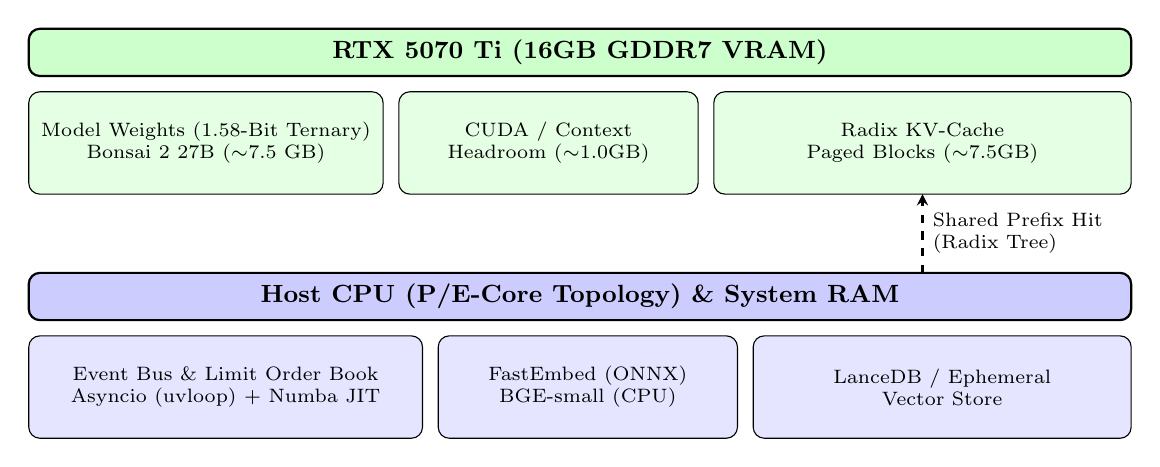
\begin{tikzpicture}[font=\sffamily]
% GPU Section
\filldraw[fill=green!20, draw=black, thick, rounded corners] (0, 0) rectangle (14, 0.6) node[midway, font=\small\bfseries] {RTX 5070 Ti (16GB GDDR7 VRAM)};
\filldraw[fill=green!10, draw=black, rounded corners] (0, -1.5) rectangle (4.5, -0.2) node[midway, align=center, font=\scriptsize] {Model Weights (1.58-Bit Ternary)\\Bonsai 2 27B ($\sim$7.5 GB)};
\filldraw[fill=green!10, draw=black, rounded corners] (4.7, -1.5) rectangle (8.5, -0.2) node[midway, align=center, font=\scriptsize] {CUDA / Context\\Headroom ($\sim$1.0GB)};
\filldraw[fill=green!10, draw=black, rounded corners] (8.7, -1.5) rectangle (14, -0.2) node[midway, align=center, font=\scriptsize] {Radix KV-Cache\\Paged Blocks ($\sim$7.5GB)};

% CPU Section
\filldraw[fill=blue!20, draw=black, thick, rounded corners] (0, -3.1) rectangle (14, -2.5) node[midway, font=\small\bfseries] {Host CPU (P/E-Core Topology) \& System RAM};
\filldraw[fill=blue!10, draw=black, rounded corners] (0, -4.6) rectangle (5, -3.3) node[midway, align=center, font=\scriptsize] {Event Bus \& Limit Order Book\\Asyncio (uvloop) + Numba JIT};
\filldraw[fill=blue!10, draw=black, rounded corners] (5.2, -4.6) rectangle (9, -3.3) node[midway, align=center, font=\scriptsize] {FastEmbed (ONNX)\\BGE-small (CPU)};
\filldraw[fill=blue!10, draw=black, rounded corners] (9.2, -4.6) rectangle (14, -3.3) node[midway, align=center, font=\scriptsize] {LanceDB / Ephemeral\\Vector Store};

% Arrow
\draw[->, >=stealth, thick, dashed] (11.35, -2.5) -- node[right, align=left, font=\scriptsize] {Shared Prefix Hit\\(Radix Tree)} (11.35, -1.5);
\end{tikzpicture}%
}
\caption{Hardware Topology and Memory Allocation across Host CPU and 16GB RTX 5070 Ti.}
\label{fig:system_topology}
\end{figure}

\begin{itemize}
    \item \textbf{Model Weights (7.5 GB):} Deploys the Qwen3.8-based \texttt{Bonsai 2 27B}, a 1.58-bit ternary hybrid-attention transformer. Critically, this model uses natively trained 1.58-bit ternary precision (\texttt{BITCOS/PQ2\_0}) optimized from initialisation, rather than post-hoc ternary quantization. The Qwen3.8 backbone features $\sim$75\% linear attention, drastically reducing the KV-cache footprint over long contexts and preventing OOM block evictions on the 16 GB RTX 5070 Ti. This establishes model cognitive reliability and GBNF/JSON schema adherence, defending the architecture against criticisms of post-hoc quantization reasoning degradation. Confining the entire parameter set to VRAM bypasses host-to-device PCIe serialisation bottlenecks entirely while unlocking massive 27B-parameter reasoning density.
    \item \textbf{Runtime \& CUDA Headroom (1.0 GB):} Reserved for CUDA context instantiation, driver overhead, and dynamic activation tensors.
    \item \textbf{Radix KV-Cache Pool (7.5 GB):} Dedicated entirely to continuous dynamic attention allocation via FP8/FP16 paged memory blocks (8-bit and 16-bit floating-point precision formats that halve memory requirements).
    \item \textbf{Offloaded Embeddings (Host CPU / Zero VRAM):} Semantic memory embeddings are served exclusively via \texttt{FastEmbed} (a lightweight execution engine for ONNX computation graphs) pinned to host CPU threads. Running \texttt{BGE-small} (a highly efficient, CPU-friendly embedding model) entirely on the CPU preserves roughly 10\% of total VRAM, preventing out-of-memory (OOM) faults during volatility-induced context spikes.
\end{itemize}

\subsection{Cognitive Serving Engine \& Radix Prefix Caching}

Agent cognition is decoupled from standard request-reply pipelines, serving batch generations via the llama-server inference engine with Slot Prefix Caching and pre-compiled structural grammars (see Figure \ref{fig:cognitive_engine}).

The core bottleneck of simulating several hundred concurrent agents is the memory footprint of the KV-Cache. Every agent must ingest the identical 2,000-token macro-environment prompt (the global news and order book state) before making a decision. If computed naively, the GPU would duplicate these 2,000 tokens in memory for every agent, instantly triggering an Out-Of-Memory (OOM) fatal error.

To solve this, the pipeline utilises Slot Prefix Caching via the PrismML-Eng/llama.cpp inference engine. Instead of treating each agent's request as an isolated generation, llama-server structures the prompts into a mathematical Radix Tree (a highly compressed prefix tree where nodes containing identical token sequences are merged). The shared 2,000-token macro environment acts as the root node of the tree and is computed and stored in the VRAM only \textit{once}. When the individual agents send their generation requests, llama-server traverses the Radix Tree, detects the identical prefix, and instantly routes all requests to read from that single cached memory block.

Broadcasting an identical 2,000-token market snapshot to all agents per tick represents a deliberate engineering trade-off: it prioritizes maximum Radix KV-cache prefix sharing over asynchronous information diffusion, trading network transmission delays for the ability to sustain 400 concurrent LLM agents on a single 16 GB GPU. Emergent herding ($H_t \to 1$) is therefore driven by persona-level heterogeneity in how each agent interprets the same shock, rather than by network topology or transmission delays. This makes the architecture academically defensible by framing prompt symmetry as a deliberate hardware optimization trade-off rather than an oversight. 

Consequently, only the highly specific, trailing tokens (the unique agent persona descriptors and their short JSON outputs) require active computation and isolated memory allocation per agent-branch. The static 2,000-token macro environment and Limit Order Book (LOB) snapshot form a single cached root node in VRAM. Variable contextual inputs--including agent personas, LanceDB RAG memories, and JSON output formatting--are strictly appended as per-agent trailing branch suffixes following the root. Macro shocks execute strictly once per episode, guaranteeing zero intra-episode root cache invalidations. The computational savings are immense:

\[ \text{Redundant FLOPs Saved} = (N - 1) \times \text{FLOPs}_{\text{prefill}}(\text{Prefix}) \]

With:
\begin{itemize}
    \item $N$: The number of concurrent LLM agents making simultaneous inference requests.
    \item $\text{FLOPs}_{\text{prefill}}(\text{Prefix})$: The floating-point operations required to perform the dense prefill (matrix multiplications) on the 2,000-token shared macro-environment.
\end{itemize}

\textbf{KV-Cache Capacity Calculation:} For a 27B model utilising Grouped-Query Attention ($L = 46$ layers, $H_{kv} = 16$ heads, $D_h = 128$) with FP8 KV-caching ($1\text{ byte per element}$):
    
\[ \text{Memory per Token} = 2 \times L \times H_{kv} \times D_h \times 1 = 188,416\text{ bytes} \approx 184\text{ KB} \]
    
With:
\begin{description}
    \item[$L = 46$] The total number of Transformer blocks/layers in the 27B model.
    \item[$H_{kv} = 16$] The number of Key-Value attention heads (utilising Grouped-Query Attention).
    \item[$D_h = 128$] The embedding dimension per attention head.
    \item[Multiplier $2$] Accounts for storing both the Key and Value matrices.
    \item[Multiplier $1$] Reflects the byte-size of the FP8 quantisation format (1 byte per parameter).
\end{description}
    
A 7.5 GB KV-cache budget yields storage for approximately:
    
\[ \frac{7.5 \times 1024^3\text{ bytes}}{188,416\text{ bytes/token}} \approx 42,740\text{ tokens} \]
    
With the 2,000-token macro prompt evaluated once ($359\text{ MB}$ total), the 7.5 GB KV-cache budget can sustain approximately $42{,}740 / 100 \approx 400$ concurrent agent branches (averaging 100 unique generation tokens each) before triggering block eviction. Sustaining a full swarm of 1,000 agents would require a $\sim$18 GB KV-cache, exceeding the hardware ceiling; the core simulation engine therefore strictly operates with $N_{\text{active}} = 400$ active LLM agents per tick.
    
\textbf{Zero-Overhead Constrained Decoding:} Agent actions must parse cleanly as structured order tickets. In a traditional pipeline, enforcing JSON output relies on post-generation validation (e.g., Pydantic throwing an error and triggering an expensive re-prompt). To solve this, the serving engine invokes GBNF/JSON schema constrained decoding compiled directly into llama-server. By pre-compiling Pydantic action schemas into finite-state machine (FSM) token masks, invalid tokens are mathematically rejected at the logit level during CUDA generation. The model is physically forced to output valid JSON matching the schema, completely eliminating retry latency and token waste.
    
\textbf{The Reflexion Cognitive Loop:} To preserve the KV-cache budget, high-frequency per-tick inline critique loops are deliberately avoided. Instead, a Reflexion-style review is staggered across ticks: rather than reviewing all 400 agents simultaneously at a global tick-50 barrier (which would cause a severe computational spike of concurrent LanceDB retrievals and LLM calls), approximately 8 agents are reviewed per tick on a rolling schedule. This distributes the reflexion overhead evenly across the tick stream, prevents latency spikes on Prometheus dashboards, and avoids false-positive SLA violations in telemetry. Intra-tick persona constraints are enforced directly through the primary prompt (e.g., explicit persona rules in the system message), eliminating the need for multi-turn self-correction during live trading.

\begin{lstlisting}[language=Python]
from pydantic import BaseModel, Field
from typing import Literal

class AgentMarketAction(BaseModel):
    agent_id: str
    action: Literal["LIMIT_BUY", "LIMIT_SELL", "MARKET_BUY", "MARKET_SELL", "HOLD"]
    volume: float = Field(gt=0.0, description="Order quantity")
    limit_price: float | None = Field(default=None, description="Mandatory if LIMIT order")
    panic_intensity: float = Field(ge=0.0, le=1.0, description="Internal affective state")
    rationale: str = Field(max_length=120, description="Bounded reasoning trace")
\end{lstlisting}

\begin{figure}[t]
\centering
\resizebox{\textwidth}{!}{%
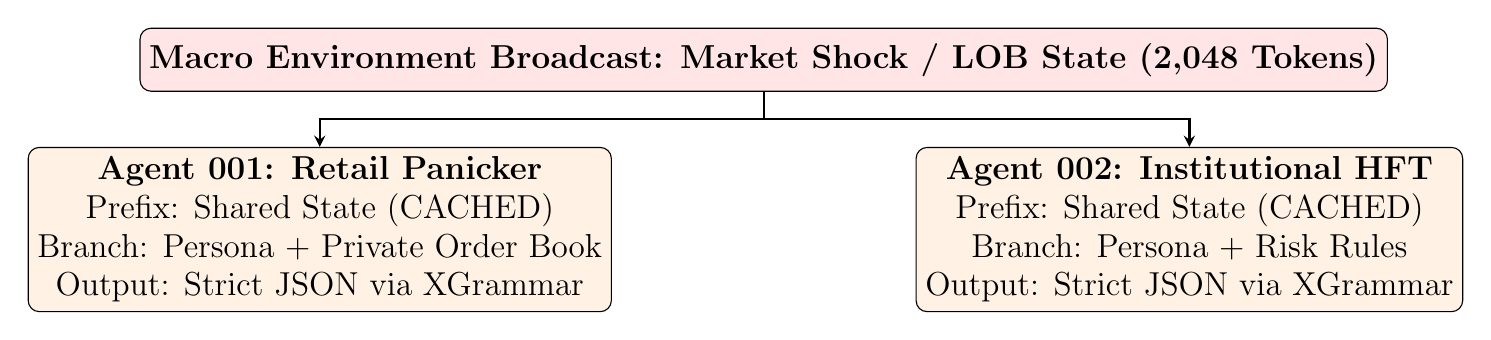
\begin{tikzpicture}[
    box/.style={draw, rectangle, rounded corners, align=center, font=\large, minimum height=1.5cm},
    macro/.style={draw, rectangle, rounded corners, fill=red!10, font=\large\bfseries, minimum width=10cm, minimum height=0.8cm},
    agent/.style={box, fill=orange!10, minimum width=6cm},
    arrow/.style={->, >=stealth, thick}
]

\node[macro] (broadcast) {Macro Environment Broadcast: Market Shock / LOB State (2,048 Tokens)};

\node[agent, below left=0.7cm and -6cm of broadcast] (agent1) {\textbf{Agent 001: Retail Panicker}\\ Prefix: Shared State (CACHED) \\ Branch: Persona + Private Order Book \\ Output: Strict JSON via XGrammar};

\node[agent, below right=0.7cm and -6cm of broadcast] (agent2) {\textbf{Agent 002: Institutional HFT}\\ Prefix: Shared State (CACHED) \\ Branch: Persona + Risk Rules \\ Output: Strict JSON via XGrammar};

\draw[arrow] (broadcast.south) -- ++(0,-0.35cm) -| (agent1.north);
\draw[arrow] (broadcast.south) -- ++(0,-0.35cm) -| (agent2.north);

\end{tikzpicture}%
}
\caption{Agent Cognitive Engine utilizing Radix Prefix Caching to efficiently route identical macro-environment tokens.}
\label{fig:cognitive_engine}
\end{figure}

\subsection{Heterogeneous Compute \& Phased Inference}

Running hundreds of highly reactive micro-agents alongside a massively complex macroeconomic orchestrator normally exceeds the VRAM boundaries of consumer hardware. This project solves this via Phased Inference (Model Multiplexing) to fully utilise both system RAM and GPU VRAM:

\begin{itemize}
    \item \textbf{Phase 1 (The Macro-Orchestrator):} A large, highly capable model acts as the ``God Agent'', generating complex geopolitical news and macroeconomic shocks. To maintain the strict \$0.00 budget and 100\% local execution mandate, this is run entirely locally by pinning a quantised dense model (e.g., Llama-3.1-70B-GGUF) into the 128 GB Host CPU RAM via \texttt{llama.cpp}. A 4-bit quantised 70B model occupies $\sim$35--40 GB and requires streaming the full weight tensor through dual-channel DDR5 memory ($\sim$80--100 GB/s bandwidth) per token, yielding roughly 2--3 tokens per second. Generating a 500-token macroeconomic shock therefore takes approximately 3--4 minutes of wall-clock time. Crucially, this is acceptable because the God Agent executes strictly once per simulation episode (not once per tick), and because simulation time is decoupled from wall-clock time; the matching engine waits for the macro shock before advancing.
    \item \textbf{Phase 2 (The Micro-Agent Swarm):} The 70B model is suspended, and the 1.58-bit ternary Bonsai 2 27B model (loaded entirely in the 16 GB GPU VRAM) processes up to 400 concurrent retail agent reactions per tick -- the hardware-bounded KV-cache ceiling.
\end{itemize}

\subsection{Reinforcement Learning (RL) Distillation}

While Large Language Models (LLMs) provide unprecedented cognitive realism, calculating deep forward-passes for even 400 agents per simulation tick remains computationally intractable for truly massive, global-scale simulations. To transition from a local 400-agent environment to a cloud-scale million-agent environment, the project introduces a Reinforcement Learning (RL) distillation pipeline.

In traditional quantitative finance, Reinforcement Learning agents are fast and highly scalable, but they suffer from rigid, hand-crafted reward functions that fail to simulate human irrationality or emotional contagion during a market crash. Conversely, LLMs perfectly capture bounded rationality and panic, but they are far too slow. By combining the two, we aim to distil the slow, high-fidelity reasoning of the LLM into a fast, lightweight RL policy.

The framework establishes the LLM as the ultimate ``Reward Signal.'' Instead of manually defining a mathematical reward for the RL agents (e.g., maximising absolute profit), we deploy the 400 generative LLM agents to trade through a simulated crisis, saving their exact decision traces and order histories to disk. 

Subsequently, we initialize lightweight, neural-network-based RL agents and train them using Proximal Policy Optimization (PPO) -- an industry-standard, highly stable reinforcement learning algorithm originally used to train ChatGPT. The loss function of the PPO algorithm is designed to penalise the RL agents whenever their actions deviate from the historical decisions made by the LLM agents under the exact same market conditions. Through thousands of training episodes, the RL policy learns to perfectly mimic the nuanced, irrational panic patterns of the generative models. 

Once the policy has converged, the heavy LLMs can be entirely decommissioned. The distilled PPO policy takes as input a fixed-size state vector $[\text{LOB\_features},\, \mathbf{e}_{\text{news}},\, \mathbf{e}_{\text{persona}}]$, where $\mathbf{e}_{\text{news}}$ is a dense embedding generated once per tick on the CPU via FastEmbed, and $\mathbf{e}_{\text{persona}}$ is a fixed agent-type embedding (e.g., retail panic trader, institutional hedger) that preserves the heterogeneous behavioural diversity of the original LLM swarm. Without $\mathbf{e}_{\text{persona}}$, a single global policy would regress to the mean of the entire swarm, collapsing the heterogeneous panic dynamics the generative models were introduced to capture. This preserves microsecond inference while retaining both qualitative conditioning on narrative shocks and persona-specific reaction profiles, allowing the macro-simulation to scale to millions of participants.

\subsection{Meso-Scale Matching Engine \& Non-Blocking Event Bus}

Simulations avoid heavy distributed coordinators such as Ray or Kafka, instead utilising a single-node asynchronous pipeline powered by Python 3.12, uvloop, and in-process shared memory buffers.

\textbf{The Event Bus (uvloop):} Standard Python asyncio suffers from significant event loop overhead. uvloop acts as a drop-in Cython replacement built on top of libuv (the same engine powering Node.js). It provides a massive throughput increase for socket I/O, which is strictly necessary to route thousands of concurrent agent actions without bottlenecking the market tick rate.

\begin{itemize}
    \item \textbf{Asynchronous Dispatch:} An asyncio.Queue event bus ingests generated agent payloads. Worker tasks batch agent decisions into discrete simulation ticks, where $t \to t+1$ advances only once the full agent cohort response has been collected. Orders within the same tick have no meaningful microsecond precedence; within-tick priority is resolved deterministically via pro-rata allocation (equal-priced limit orders share execution proportionally by volume), eliminating latency arbitrage from Python task-scheduling jitter.
    \item \textbf{Algorithmic Market Makers (Equilibrium Baseline):} To prevent immediate model collapse, the order book is populated by Inventory-Aware Market Makers using a simplified Avellaneda-Stoikov model, with a hard inventory bound $|q| \le Q_{\text{limit}}$. These background scripts dynamically adjust their reservation prices ($P_{\text{reservation}} = P_{\text{mid}} - \gamma \cdot q \cdot \sigma^2$) to protect against adverse selection. Critically, once inventory $q$ reaches $Q_{\text{limit}}$, the market maker ceases posting bid (or ask) quotes entirely, modelling real-world liquidity withdrawal and flash-crash black holes.
    \item \textbf{Frequent Batch Auction (Call Market) Engine:} To prevent Python's Global Interpreter Lock (GIL) from bottlenecking high-throughput market clearing, the matching engine operates as a discrete Frequent Batch Auction clearing at the $t \to t+1$ tick boundary using compiled, memory-contiguous arrays (via Numba JIT with \texttt{@jit(nopython=True, cache=True)}). Enabling Numba's on-disk cache avoids the multi-second cold-start compilation delay on the first tick; a pre-warmed dummy dispatch is also executed before metric logging begins to prevent tick-0 telemetry outliers. All 400 agent orders generated during tick $t$ are aggregated into an auction batch. The engine calculates a single, uniform market-clearing price that maximizes total crossed volume, allocating executed quantities among equal-priced orders via pro-rata volume distribution. This completely eliminates continuous price-time priority and latency arbitrage.
    
    \item \textbf{Ephemeral State (Redis):} Because the LOB tick clock advances only after the full agent cohort responds, the market state during any generation phase is perfectly static. The canonical tick-$t$ market snapshot (best bid, best ask, LOB depth) is therefore injected once into the shared Radix prompt prefix at the start of each tick, eliminating mid-tick Redis queries from the critical path entirely. Redis is retained exclusively for inter-process coordination, writing the final cleared prices and inventory snapshots at $t+1$ so that the next tick's prefix can be assembled by the event bus.
    
    \item \textbf{Long-Term Semantic Memory (LanceDB):} As agents execute trades, they generate textual rationales (e.g., ``I am panic selling because liquidity is drying up''). Storing this string data for hundreds of agents entirely in RAM causes fatal memory bloat. LanceDB acts as an embedded, serverless vector database that streams these rationales to disk as semantic embeddings. Agents can then perform lightning-fast similarity searches (RAG) over their past memories without crashing the Python process. Because LanceDB performs synchronous Apache Arrow disk operations, all database calls are wrapped in \texttt{asyncio.to\_thread()} to offload them onto a dedicated thread pool, preventing disk I/O from blocking the \texttt{uvloop} event thread and introducing artificial latency into the tick cycle. RAG lookups are batched into a single vectorised query per tick boundary rather than issuing 400 individual async calls.
\end{itemize}

\subsection{Production Deployment \& Telemetry Stack}

The infrastructure deploys via standard containerisation to minimise setup overhead and eliminate bare-metal OS configuration fragility. Table \ref{tab:telemetry_stack} outlines the complete deployment stack.

\begin{table}[b]
\centering
\caption{Production Deployment and Telemetry Runtime Configuration.}
\label{tab:telemetry_stack}
\renewcommand{\arraystretch}{1.3}
\begin{tabular}{|l|l|p{6cm}|}
\hline
\textbf{Layer} & \textbf{Component} & \textbf{Runtime Configuration / Flags} \\ \hline
\textbf{Base OS} & Ubuntu 24.04 LTS Bare-Metal & Standard kernel, NVIDIA Driver 550+, Docker CE \\ \hline
\textbf{Macro-Orchestrator} & Host CPU & \texttt{llama.cpp} with 70B GGUF model pinned to 128GB RAM \\ \hline
\textbf{Acceleration} & NVIDIA Container Toolkit & Direct GPU passthrough via \texttt{cdi} / \texttt{--gpus all} \\ \hline
\textbf{Serving Node} & llama-server Docker Container & \texttt{--model-path <bonsai\_2\_27b> --dtype int2 --mem-fraction-static 0.90} \\ \hline
\textbf{Pipeline Core} & Python 3.12 (pixi) & \texttt{uvloop}, \texttt{pydantic-core}, \texttt{lancedb}, \texttt{numba} \\ \hline
\textbf{Telemetry} & Prometheus \& Grafana & Scraping llama-server \texttt{/metrics} and custom LOB drift collectors \\ \hline
\end{tabular}
\end{table}

\begin{itemize}
    \item \textbf{LLMOps Telemetry \& Token SLAs:} Because simulation time is decoupled from wall-clock time, the tick clock advances only after the full agent batch completes. The telemetry layer instead tracks generation latency as a first-class simulation throughput metric rather than a hard real-time deadline. We track:
    \begin{itemize}
        \item \textbf{TTFT (Time-To-First-Token):} The latency between the event bus dispatching the prompt and llama-server yielding the first decision token.
        \item \textbf{ITL (Inter-Token Latency):} The speed at which subsequent JSON characters are streamed back to the parser.
        \item \textbf{Schema Failure Rate:} The percentage of ticks where an agent failed to return a valid action.
    \end{itemize}
    \item \textbf{Systemic Drift Monitoring:} Tracks emergent behaviour in order to differentiate realistic financial contagion from model hallucinations:
    \begin{itemize}
        \item \textbf{Herding Index ($H_t$):} Measures behavioural clustering across agent actions:
        
        \[ H_t = \left\vert{} \frac{\sum Q_{t}^{\text{buy}} - \sum Q_{t}^{\text{sell}}}{\sum Q_{t}^{\text{buy}} + \sum Q_{t}^{\text{sell}} + \epsilon} \right\vert{} \quad \in [0, 1] \]
        
        With:
        \begin{description}
            \item[$H_t$] The Herding Index at time $t$ ($0$ = perfectly balanced market, $1$ = absolute panic/herding in a single direction).
            \item[$\sum Q_{t}^{\text{buy}}$ / $\sum Q_{t}^{\text{sell}}$] The aggregate volume of buy and sell orders crossing the spread at exactly tick $t$.
            \item[$\epsilon$] A minuscule constant (e.g., $10^{-7}$) injected to prevent mathematical undefined behaviour (division by zero) during periods of zero trading volume.
        \end{description}
        
        \item \textbf{Entropy of Rationale Embeddings:} Computes the dispersion of agent reasoning embeddings via LanceDB to detect semantic collapse (where all agents begin repeating identical panic phrases regardless of their assigned persona).
    \end{itemize}
\end{itemize}

\section{MLOps, CI/CD, \& Quality Assurance Strategy}

To ensure the mathematical soundness of the simulation while maintaining a strict delivery timeline, the project employs a streamlined, high-impact lean strategy:

\begin{enumerate}
    \item \textbf{Local Self-Hosted GitHub Actions Runner:} Automate linting (\texttt{ruff}), secret scanning (\texttt{gitleaks}), Pydantic contract tests, and Numba LOB invariant verification (\texttt{Hypothesis}) directly on the local Ubuntu 24.04 server on every \texttt{git push}.
    \item \textbf{Single-Command Containerization:} Use \texttt{docker compose up} to seamlessly orchestrate llama-server, FastAPI, Redis, and Prometheus without heavy cloud dependencies.
    \item \textbf{Local DVC Data Versioning:} Version market seeds, order book states, and prompt files using DVC backed by local disk storage (\texttt{/var/dvc\_store}).
    \item \textbf{Prometheus \& Grafana Observability:} Track 4 core operational and financial metrics: Time-To-First-Token (TTFT), Inter-Token Latency (ITL), Active Agent Count ($N_{\text{active}}$), and the Herding Index ($H_t$).
    \item \textbf{Explicit Scope Simplification:} Explicitly exclude heavy orchestrators (e.g., Airflow, MinIO, Postgres databases) in favor of lightweight local equivalents, utilizing embedded local-file MLflow tracking (\texttt{backend\_store\_uri="./mlruns"}) with zero server overhead. This keeps development time focused on engine execution and eliminates 30--40 hours of unnecessary DevOps infrastructure maintenance within the 160-hour execution window.
\end{enumerate}

\section{Project Timeline \& Graceful Degradation Strategy}

Given the strict 2-month (approximately 160 hours) core execution window, the project employs a "Graceful Degradation" strategy. This ensures that a fully compliant, production-grade MLOps deliverable is ready at the earliest milestone, treating the most computationally unstable features as stretch goals.

\subsection*{Phase 1: Bare-Metal Infrastructure \& Minimum Viable MLOps Product (Weeks 1--4 | $\sim$90 Hours)}
\begin{itemize}
    \item \textbf{Goal:} Provision the physical server and pass the core MLOps requirements by deploying a fully functional, containerised LLM trading pipeline.
    \item \textbf{Scope:} 
    \begin{itemize}
        \item \textit{DevOps \& Infrastructure:} Bare-metal provisioning of Ubuntu 24.04, securing network access via Tailscale, kernel-level blacklisting of \texttt{nouveau} drivers, and installing the proprietary NVIDIA 550+ CUDA stack with \texttt{nvidia-container-toolkit} for Docker GPU passthrough.
        \item \textit{Core Systems:} Building the strictly reproducible \texttt{pixi} environment, constructing the Numba-JIT Limit Order Book (LOB), and setting up the \texttt{uvloop} asynchronous event bus with Redis and LanceDB connections.
        \item \textit{LLM Inference:} Deploying the llama-server container, downloading and serving the quantised models, tuning the KV-Cache memory fraction to \texttt{--mem-fraction-static 0.90} (allocating $\sim$14.4 GB to llama-server and preserving $\sim$1.6 GB of VRAM safety headroom for CUDA drivers and GBNF FSM table allocations), and implementing GBNF/JSON constrained schemas.
        \item \textit{Development Strategy:} During integration testing and debugging, a lightweight proxy model (e.g., Llama-3.1-8B or Mistral-7B-Instruct) replaces the 70B God Agent to eliminate multi-minute CPU prefill latency from iteration loops. The full 70B model is reserved exclusively for final production benchmark runs. The simulation engine and Numba LOB are prioritised for end-to-end integration before investing time in advanced telemetry, \texttt{mutmut} mutation sweeps, or Grafana dashboard fine-tuning.
    \end{itemize}
    \item \textbf{Deliverable:} Up to 400 concurrent LLM agents (the hardware-bounded KV-cache ceiling for the 27B model on 7.5 GB) successfully routing structured JSON trades through the event bus. A live Prometheus/Grafana telemetry dashboard tracking ITL, TTFT, and the emergent Herding Index.
\end{itemize}

\subsection*{Phase 2: Heterogeneous Compute \& Orchestration (Weeks 5--6 | $\sim$40 Hours)}
\begin{itemize}
    \item \textbf{Goal:} Elevate the project architecture by multiplexing both the CPU and GPU for different LLM tasks.
    \item \textbf{Scope:} Implementing the Phased Inference logic. Orchestrating the "God Agent" macro-orchestrator (pinned strictly in the 128GB Host CPU RAM via Llama.cpp) to generate macroeconomic shocks, which then seamlessly triggers the 27B micro-agent swarm (pinned strictly in the 16GB GPU VRAM) to react.
    \item \textbf{Deliverable:} Proof of advanced hardware orchestration and extreme cost-efficiency on a \$0.00 compute budget, demonstrating that massive multi-agent simulations can run locally without cloud dependencies.
\end{itemize}

\subsection*{Phase 3: RL Distillation Stretch Goal (Weeks 7--8 | $\sim$30 Hours)}
\begin{itemize}
    \item \textbf{Goal:} The high-risk, high-reward research phase to scale the simulation from 400 to 1,000,000 agents.
    \item \textbf{Scope:} Formatting the simulation as an OpenAI Gym environment. Utilising Ray RLlib or Stable Baselines3 to train lightweight Proximal Policy Optimization (PPO) neural networks, using the saved LLM reasoning traces as the ultimate reward signal. Critically, scaling to one million agents requires replacing the Python \texttt{uvloop} meso-layer with a fully compiled aggregation backend (e.g., a Rust-based order router or Numba-JIT parallel dispatch), as routing one million asynchronous payloads through a single Python event loop per tick would catastrophically saturate the GIL and render the simulation non-functional at this scale.
    \item \textbf{Risk Mitigation:} Because RL tuning is notoriously unstable, this phase acts strictly as a stretch goal. Should policy distillation fail to converge before the deadline, the project gracefully degrades to submitting the completed Phase 2 architecture.
\end{itemize}

\section{Deliverables \& Evaluation Criteria}

\begin{enumerate}
    \item \textbf{System Architecture Document:} Complete specification of the event bus, memory architecture, and clearing engine logic.
    \item \textbf{Reproducible Simulation Pipeline:} Containerised deployment (Docker/Compose) enabling single-command execution.
    \item \textbf{MLOps Dashboard:} Live monitoring panel displaying serving telemetry (TTFT, throughput), JSON parsing error rates, and emergent macro market indices.
    \item \textbf{Experimental Backtest Report:} A comparative analysis contrasting standard rule-based financial models against the generative agent framework during simulated liquidity shocks.
\end{enumerate}

\section{Coverage of Course Requirements}

To align with the expected MLOps curriculum phases, the project fulfils the standard milestones as follows:

\begin{itemize}
    \item \textbf{Phase 1 (Foundations):} Containerised llama-server environment via Docker; explicit system objectives and throughput metrics defined.
    \item \textbf{Phase 2 (Build \& Tracking):} End-to-end pipeline connecting the uvloop event bus to llama-server; Local DVC Data Versioning for market seeds and prompts, embedded local-file MLflow tracking for generative model runs (\texttt{backend\_store\_uri="./mlruns"}), Phased Inference parameter sweeps, and prompt registry versioning.
    \item \textbf{Phase 3 (Deployment):} Asynchronous serving of the simulation ticks; storage of simulation artefacts and memory states in LanceDB and Redis.
    \item \textbf{Phase 4 (Monitoring):} Grafana dashboards for serving telemetry (TTFT, latency); drift detection for agent behaviour distributions during simulated market crashes.
\end{itemize}

\section{Risks \& Fallbacks}

\begin{itemize}
    \item \textbf{RL Non-Convergence (Highest Risk):} Reinforcement learning is notoriously unstable and sensitive to reward shaping. Should the PPO agents fail to mimic the LLM traces within the timeframe, the fallback is to simply omit Phase 3 and present the Phase 2 Phased Inference architecture as the finalised project.
    \item \textbf{VRAM Exhaustion (OOM):} Should the 16GB limit be breached during high-concurrency spikes, the fallback is to aggressively lower the uvloop concurrency limit or shrink the Radix KV-Cache pool.
\end{itemize}

\section{GDPR, Security \& Ethics}

\begin{itemize}
    \item \textbf{Financial Advice Disclaimer:} The simulation is strictly an academic sandbox for testing MLOps pipelines. It is explicitly not intended for, and cannot provide, real-world financial or investment advice.
    \item \textbf{Data Privacy:} The system relies solely on synthetic data and public macro-economic indicators. No personal data or proprietary trading histories are utilised.
    \item \textbf{Secrets Management:} Any required API keys (e.g. for fetching live economic data) are injected via environment variables and excluded from version control, reinforced by secret scanning in CI.
\end{itemize}

\section{Data \& Bibliography}

\subsection*{Data Sources}
\begin{itemize}
    \item \textbf{FRED (Federal Reserve Economic Data):} For parameterising baseline macroeconomic states (e.g. interest rates, volatility indices).
    \item \textbf{Synthetic Order Book Generation:} Initial state distributions drawn from standard statistical financial models. Background order arrivals follow a Poisson process, and the limit prices are distributed using an exponential density function centered around a fundamental mid-price.
\end{itemize}

\subsection*{Bibliography}
\begin{itemize}
    \item Sculley et al., \textit{Hidden Technical Debt in Machine Learning Systems} (NeurIPS 2015).
    \item Breck et al., \textit{The ML Test Score: A Rubric for ML Production Readiness and Technical Debt Reduction}.
    \item López de Prado, \textit{The 10 Reasons Most Machine Learning Funds Fail}.
\end{itemize}

\end{document}
